% figures/dynamics/schwerpunkt_trajectory-DE.tex
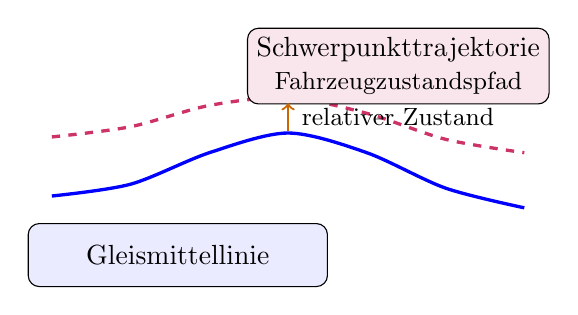
\begin{tikzpicture}[
  x=1cm,y=1cm,
  box/.style={draw, rounded corners, align=center, minimum width=3.8cm, minimum height=0.8cm}
]
\draw[very thick, blue] plot[smooth] coordinates {(0,0) (1,0.15) (2,0.55) (3,0.8) (4,0.55) (5,0.1) (6,-0.15)};
\draw[very thick, purple!80, dashed] plot[smooth] coordinates {(0,0.75) (1,0.88) (2,1.15) (3,1.25) (4,1.05) (5,0.72) (6,0.55)};

\node[box, fill=blue!8] at (1.6,-0.75) {Gleismittellinie};
\node[box, fill=purple!10] at (4.4,1.65) {Schwerpunkttrajektorie\\\small Fahrzeugzustandspfad};

\draw[->, thick, orange!80!black] (3,0.82) -- (3,1.18);
\node[right] at (3.05,1.0) {\small relativer Zustand};
\end{tikzpicture}
